\label{sec:background}
In diesem Kapitel werden die wichtigen Grundlagen erläutert, die nötig sind, um das Problem mangelhafter Softwaredokumentation zu lösen.  Dazu  wird der Begriff \enquote{Softwaredokumentation} genauer definiert. Außerdem wird eine Einführung in Code-Smells gegeben.  Anschließend gibt es eine Einführung in Javadoc gegeben, dessen Analyse der Schwerpunkt dieser Bachelorarbeit ist. Danach wird die \ac{CI/CD}-Plattform \enquote{GitHub Actions} präsentiert, die genutzt werden soll, um die Dokumentationsqualität regelmäßig zu messen. Am Ende werden weitere Tools vorgestellt, die fehlerhafte Dokumentationen erkennen. Außerdem werden wissenschaftliche Arbeiten zusammengefasst, die sich ebenfalls mit der Thematik \enquote{Softwaredokumentation} befassen. 
 

\hfill
\section{Softwaredokumentation}\label{chapter:documentation}
Um den Begriff \enquote{Softwaredokumentation} zu definieren, sollte zunächst der Begriff \enquote{Dokumentation} definiert werden. Das IEEE  definiert diesen Begriff als jede textliche oder bildliche Information, welche Aktivitäten, Anforderungen, Abläufe oder Ergebnisse beschreibt, definiert, spezifiziert, berichtet oder zertifiziert \cite[S. 28]{IEEEStandardGlossaryofSoftwareEngineeringTerminology}. Somit beschreibt eine Dokumentation, wie sich eine Komponente aufgebaut ist oder wie sie sich verhält.

Diese abstrakte Definition lässt sich so auf Softwareentwicklung übertragen. In \cite[S. 125]{Softwaredocumentationandstandards} wird Softwaredokumentation als eine Sammlung von technischen Informationen dargestellt, die für Menschen lesbar sind und welche die Funktionen, Benutzung oder das Design eines Softwaresystems beschreiben. So beschreibt Donald E. Knuth in \cite[S. 97]{LiterateProgramming}, dass die Hauptaufgabe beim Programmieren nicht sein sollte, einen Computer zu erklären, was er machen sollte, sondern anderen Menschen zu erklären, was der Computer machen sollte. Beispiele für Softwaredokumentation sind Kommentare,  UML-Diagramme, Readme-Dateien oder Handbücher.

Im Kontext dieser Bachelorarbeit sollen allerdings nur bestimmte Arten der Softwaredokumentation betrachtet werden, da eine umfassende Betrachtung innerhalb der vorgegebenen Zeit nicht möglich ist.  Zwar wären Readme-Dateien oder UML-Diagramme für eine Bewertung auch interessant, allerdings sind diese nicht so stark mit dem dazugehörigen Code verknüpft, sondern befinden sich in externen Dateien, sodass eine Verarbeitung ungleich schwieriger wäre.

Aus diesem Grunde konzentriert sich diese Bachelorarbeit nur auf Kommentare. Studien zeigen, dass Kommentare eine hohe Relevanz in der Softwareentwicklung haben, sodass eine Analyse der Kommentare eine gute Annäherung an die tatsächliche Qualität der Dokumentation geben kann \cite[S. 71]{AStudyoftheDocumentationEssentialtoSoftwareMaintenance}. Dabei sollen nicht alle Kommentare betrachtet werden, sondern nur eine bestimmte Kategorie von Kommentaren, die besonders leicht verarbeitbar sind, sodass aus ihnen viele Informationen extrahiert werden können und die Bewertung dadurch genauer werden kann. 

Für diese Bachelorarbeit werden daher nur bestimmte Inline-Kommentare im Quellcode betrachtet, die ein Spezialfall von normalen mehrzeiligen Kommentaren sind.
Diese Kommentare werden wie normale Kommentare erkannt und werden daher nicht Bestandteil des kompilierten Programms. Nichtsdestotrotz haben diese spezifischen Kommentare aber eine bestimmte Struktur, die eine leichte Verarbeitung durch Computerprogramme ermöglicht und gleichzeitig trotzdem für Menschen lesbar bleibt. In vielen Fällen werden diese Kommentare einer bestimmten Komponente zugeordnet, wobei dies dadurch geschieht, dass der Kommentar direkt vor dieser Komponente steht. 
\begin{comment}
Ein Beispiel dafür ist Javadoc, da jeder Javadoc-Kommentar auch ein gültiger mehrzeiliger Kommentar ist.
\end{comment}




\section{Code-Smells}\label{chapter:code_smell}
Der Begriff \enquote{Code-Smell} (z.~dt. übel riechender Code)  wurde von Kent Beck in \cite[S. 71 ff.]{fowler2019refactoring}  vorgeschlagen, um Quellcode zu beschreiben, bei dem Refactoring (z.~dt. Restrukturierung) sinnvoll ist. Bestimmte Strukturen im Quellcode deuten darauf hin, dass der Code verbessert werden sollte, da ansonsten die zukünftige Wartbarkeit des Codes verringert wird. Beispiele sind schlecht gewählte Namen für Variablen oder Methoden, duplizierter Code, lange Methoden oder globale Daten. In bestimmten Situationen werden Kommentare ebenfalls als Code-Smell klassifiziert, da sie auf komplizierten  Code hindeuten können oder der Name einer Komponente schlecht gewählt wurde. Daher sollte geprüft werden, ob nach einem Refactoring die Kommentare noch notwendig sind.

Nach \cite[S. 249-250]{JavadocViolationsandTheirEvolutioninOpen-SourceSoftware} kann eine mangelhafte Dokumentation als Code-Smell bezeichnet werden, da sie die Wartbarkeit der Software beeinträchtigen kann. Dies gilt besonders, wenn die Dokumentation vom Code abweicht und damit bei den Entwicklern zu Verwirrung führt. Eine fehlerhaft dokumentierte Methode, bei der beispielsweise ein Parameter nicht dokumentiert ist, deutet stark auf Code-Smells hin, da der Code von der Dokumentation divergiert. Zudem kann eine \ac{IDE} die Informationen von strukturierten Kommentaren nutzen, um beispielsweise den Benutzer einer Methode Hinweise zur Benutzung zu geben. Dies ist bei normalen Kommentaren nicht möglich. 

\section{Javadoc}\label{chapter:javadoc}
Javadoc \cite{HowtoWriteDocCommentsfortheJavadocTool} ist ein Tool zur Generierung von Dokumentationen, das sich als de facto Standard für Dokumentationen in der Programmiersprache Java etabliert hat \cite[S. 249]{JavadocViolationsandTheirEvolutioninOpen-SourceSoftware}.  Javadoc besteht aus speziellen Java-Kommentaren, die an bestimmten Stellen im Quellcode eingefügt werden und daher bei der Kompilation nicht berücksichtigt werden. Ein Javadoc-Block beschreibt immer ein bestimmtes Modul (z. B. eine Klasse, Methode oder Feld). Es beginnt mit der Zeichenkette \enquote{/**}, wobei die ersten beiden Zeichen \enquote{/*} den Beginn eines mehrzeiligen Kommentars in Java einläuten, und endet mit \enquote{*/}. Durch das zusätzliche \enquote{*} unterscheidet sich ein Javadoc-Kommentar von einem normalen mehrzeiligen Kommentar, der zwar zur Kommentierung eines Blocks verwendet werden kann, aber vom Javadoc-Tool ignoriert wird und daher einen geringeren Mehrwert hat. 


		\begin{figure}[ht!]
			\lstinputlisting
			[caption={Beispielhafter Javdoc-Block für einfache Methode},
			label={lst:simple_javadoc},
			captionpos=b,language=java, basicstyle=\footnotesize, tabsize=1, showstringspaces=false,  numbers=left]
			{figures/chapter2/ternary.java}
		\end{figure}

Listing \ref{lst:simple_javadoc} zeigt ein Beispiel für eine gelungene Verwendung von Javadoc. Zunächst wird der Zweck der Methode beschrieben, anschließend wird jeder Parameter erläutert. Dabei sollte in komplexeren Fällen auch erklärt werden, welche Werte gültig für den Parameter sind. Danach folgt eine Beschreibung des Rückgabewertes, welche am besten auch jeden möglichen Fall abdeckt. Mit \enquote{{@code ...}} kann auf einen Parameter referenziert werden. Mit diesen Informationen kann der Programmierer leicht überblicken, wie eine Methode genutzt werden, sodass die Einarbeitungszeit und die Fehleranfälligkeit reduziert werden kann.  

		
		
Zunächst sollte am Anfang des Blocks eine generelle Zusammenfassung der Komponente geschrieben werden. Danach können sogenannte Tags (z.~dt. Auszeichner), die mit dem \enquote{@}-Zeichen beginnen, benutzt werden. Diese beschreiben wiederum einen bestimmten Teilbereich einer Komponente. Es ist zudem Konvention, dass jede Zeile in einem Javdoc-Block mit einem Asterisk beginnt. 

In der folgenden Auflistung werden beispielhaft einige Javadoc-Tags aufgelistet und beschrieben:
\begin{description}
         \item[@param]  Beschreibt einen Parameter, benötigt den Parameternamen als Argument
         \item[@return]  Beschreibt den Rückgabewert der Methode, sofern er existiert 
         \item[@throws] Beschreibt welche Ausnahmen diese Methode werfen kann und möglichst unter welchen Umständen dies passiert, benötigt den Namen der Ausnahme. Für mehrere Ausnahmen sollte dieser Tag entsprechend wiederholt werden 
         \item[@deprecrated] Falls diese Methode veraltet ist und nicht mehr verwendet werden sollte, kann hier eine Alternative beschrieben werden. 
        
\end{description}



Diese Javadoc-Blöcke können dann von dem gleichnamigen Tool in eine HTML-Datei umgewandelt werden und ermöglichen den Entwicklern damit einen komfortablen Überblick über alle Komponenten eines Moduls. Zudem könne Javadoc-Blöcke ebenfalls HTML-Inhalte besitzen, die dann von Javadoc in die HTML-Datei übernommen werden, sodass der Entwickler beispielsweise Tabellen zur übersichtlichen Präsentation  von Informationen verwenden kann. 

Eine \ac{IDE} kann die Informationen auslesen und dann beispielsweise bei der Autovervollständigung nutzen, um den Entwickler beim Schreiben des Programmcodes unterstützen. So kann sich ein Programmierer auch in einer fremden \ac{API} leichter zurechtfinden.

Ein Javadoc-Kommentar wird vererbt und muss daher für eine abgeleitete Klasse nicht neu geschrieben oder redundant geklont werden. Dies ist sinnvoll, da abgeleitete Klassen einen Vertrag erfüllen müssen, der bei einer guten Dokumentation auch schon in der Javadoc-Dokumentation beschrieben wird. Auch bei Methoden, die aufgrund einer Schnittstelle implementiert werden müssen, ist eine Neudefinition des Javadoc-Kommentar unnötig. Falls sinnvoll, kann aber dennoch ein eigener Javadoc-Kommentar erstellt werden, der allerdings den Kommentar der Quelle vollständig ersetzt. Mit \textit{@inheritDoc} kann der ursprüngliche Kommentar aber trotzdem eingefügt werden.

Nachfolgend ist ein Auszug von empfehlenswerten Tipps von der Oracle-Webseite, die beim Schreiben von Javadoc beachtet werden sollten \cite{HowtoWriteDocCommentsfortheJavadocTool}:
\begin{itemize}
    \item Nicht in jedem Fall vollständige Sätze verwenden, aber klar formulieren, was die Aufgabe einer Komponente ist
    \item In der dritten und nicht in der zweiten Person schreiben
    \item Nicht repetitiv sein. Ein Kommentar, der im Wesentlichen nur den Namen einer Komponente wiedergibt, hat keinen Mehrwert
    \item  Beschreibungen von Methoden sollten mit einem Verb beginnen
    \item Keine lateinischen Ausdrücke wie \enquote{e.g}, \enquote{aka} oder \enquote{i.e} verwenden
    \item Bei einem Verweis auf das aktuelle Objekt sollte das spezifische \textit{this} statt des allgemeineren \textit{the} verwendet werden, bspw. \enquote{opens the connection of \textbf{this} object} statt \enquote{opens the connection of \textbf{the} object}
    \item Bezeichner sollten mit \textit{<code></code>} umschlossen werden, um deutlich zu machen, dass dies eine andere Komponente ist
    \item Der Kommentar sollte eventuelle Unterschiede unter verschiedene Plattformen erläutern
    \item Die Dokumentation sollte erläutern, wie sich die Komponente in Randfällen verhält
    
\end{itemize}

Für andere Programmiersprachen gibt es vergleichbare Werkzeuge, die ähnliche Funktionen anbieten und bei denen die Dokumentationen mit einer relativ ähnlichen Syntax erstellt werden. Dazu gehören beispielsweise Doxygen für C++-Programme oder der PHP-Documentor für PHP-Programme. 


\section{JavaScript, Node und TypeScript}
Das Tool wird mittels der \textit{Node.js}-Bibliothek und TypeScript entwickelt.
In diesem Abschnitt werden daher die grundlegenden Programmiersprachen und Bibliotheken vorgestellt, die zur Entwicklung des Tools als Desktopanwendung notwendig sind. Außerdem wird begründet, warum TypeScript und \enquote{Node.js} für die Entwicklung des Tools verwendet wurden. 
\subsubsection{JavaScript}
JavaScript ist eine dynamisch typisierte Programmiersprache, die sich als de facto Standard  für Browserskripte etabliert hat, die auf dem Client (z.~dt. Klienten) ausgeführt werden. Zum Beispiel lassen sich mittels JavaScript Webseiten dynamisieren, Eingaben von Formularen validieren oder nachträglich Daten von anderen Servern laden. 

Die Syntax von JavaScript basiert wie bei der Programmiersprache Java auf C, dennoch sollten Java und JavaScript nicht verwechselt werden. Die eingangs erwähnte dynamische Typisierung bedeutet im Gegensatz zur statischen Typisierung, dass eine Variable anders als in Java keinen fixen Datentyp hat, sondern der Datentyp sich stets nach den aktuellen Wert richtet. Eine Variable \textit{foo} kann mit dem Befehl \textit{ let foo = true} deklariert werden und ist dann vom Datentyp \textit{Bool}. Daraufhin kann der gleichen Variable eine Zeichenkette zugewiesen werden, sodass die Variable nun vom Datentyp \textit{String} ist. Durch die dynamische Typisierung ist der Programmierer flexibler, jedoch zeigt eine Studie, dass die Softwarequalität bei Projekten mit statischer Typisierung etwas besser ist als mit dynamischer Typisierung\cite[S. 155ff.]{Ray2014}.

\subsubsection{TypeScript}
TypeScript ist eine auf JavaScript aufbauende Programmiersprache, die JavaScript um statische Typisierung ergänzt. Jeder JavaScript-Code ist gültiger TypeScript-Code, sodass TypeScript als Obermenge von JavaScript angesehen werden kann. Der TypeScript-Code kann nicht direkt ausgeführt werden, sondern wird in gültiges JavaScript transkribiert, sodass er von einem Client mit JavaScript-Unterstützung ausgeführt werden kann. 

In TypeScript können Typannotationen verwendet werden, die den Datentyp einer Variablen festlegen. Eine Variable \textit{foo} kann in TypeScript dem Befehl \textit{let foo:boolean=true} als \textit{Boolean} deklariert werden. Durch die Angabe \enquote{:boolean} ist der Datentyp fix und kann nicht geändert werden. Eine Zuweisung einer Zeichenkette zu \textit{foo} würde TypeScript mit einer Fehlermeldung quittieren. Auch viele Funktionen, die in objektorientierten Programmiersprachen verbreitet sind, wie z.~B. Schnittstellen, generische Typen oder Namensräumen werden von TypeScript unterstützt und helfen so dabei, komplexere Programme zu schreiben. Aus diesen Gründen wurde TypeScript gewählt, denn eine Verwendung von statischen Typen und anderen objektorientierten Funktionen ermöglicht eine bessere Abstraktion der einzelnen Schritte (Traversierung, Parsing, Anwendung der Metriken etc.). 

\subsubsection{Node.js}
Die Bibliothek  \textit{Node.js} ist eine beliebte Bibliothek, um JavaScript-Programme nicht nur im Browser, sondern auch als eigenständige Applikation zu programmieren. Dadurch haben sie im Gegensatz zu den klassischen Browser-Skripten freien Zugriff auf das Dateisystem und Netzwerkfunktionen.  Die Bibliothek läuft auf den meisten Systemen und  wird von GitHub Actions nativ unterstützt. Außerdem gibt es über dem Paketmanager \textit{NPM} eine große Auswahl an kleineren Bibliotheken, die kleinere Probleme lösen können und damit Entwicklungsaufwand bei Aufgaben sparen, welche nicht im Kernbereich dieser Bachelorarbeit liegen; folglich wurde diese Bibliothek als Fundament für die Entwicklung des Tools genutzt. 

\section{GitHub Actions}\label{chapter:github_actions}

GitHub Actions \cite{GithubActions} ist eine von GitHub angebotene Plattform zur Vereinfachung des \ac{CI/CD}'s. Mithilfe von  GitHub Actions wird Programmcode ausgeführt, wenn ein bestimmtes Ereignis stattfindet. Dieses Ereignis kann z. B. ein Push-Ereignis sein, bei dem neuer Quellcode in das GitHub-Repository hochgeladen wird oder eine neue Version des Programms zum Release freigegeben wird. Der Programmcode kann wahlweise auf einem von  GitHub vorbereiteten System ausgeführt oder auf einem eigenen System ausgeführt werden. Dieses System wird auch als \textbf{Runner} bezeichnet.

Der gesamte Programmcode wird im Kontext von GitHub Actions auch als \textbf{Workflow (Ablauf)} bezeichnet und führt einen oder mehrere \textbf{Jobs} aus. Diese Jobs sind eine Ansammlung von \textbf{Steps (Schritte)}, die man als Befehle interpretieren kann. Die Jobs werden standardmäßig parallel ausgeführt, da keine Abhängigkeit zwischen den Jobs vermutet wird. Ein Step kann ein Befehl sein, der auf einer Kommandozeile ausgeführt werden kann, oder ein Verweis auf eine andere GitHub Action, die dann ausgeführt wird \cite[S. 5-7]{github_action_book}. 


Abbildung \ref{fig:workflow_schema} zeigt schematisch wie ein Workflow in einem GitHub-Projekt ausgeführt werden kann. Eine Benutzer löst beispielsweise durch einen Push ein Ereignis aus. Daraufhin werden für jeden Job ein Runner initialisiert, die aus dem Repository das Projekt klonen, um so mit einer geklonten Kopie zu arbeiten.  Das Klonen des Repositorys ist dabei nicht obligatorisch, ist aber notwendig, falls mit dem Quelltext des Projektes gearbeitet werden soll.  Anschließend werden die Jobs gestartet, die ihrerseits wieder die Steps ausführen. Jeder Job wird auf einen separaten Runner ausgeführt und läuft parallel, außer der Benutzer gibt explizit eine Abhängigkeit zwischen den Jobs an. 
\begin{figure}[ht!]
\fontsize{7}{10}\selectfont
    \centering
\includesvg[scale=0.8]{figures/chapter2/workflow_schema.svg}
    \caption{Schema: Workflows}
    \label{fig:workflow_schema}
\end{figure}

Schlägt der Programmcode fehl, kann der Nutzer den Grund des Fehlers über die  \enquote{Actions}-Registerkarte herausfinden. Dort kann der Nutzer auch sämtliche Ausgaben des Programms ansehen, die auf der Konsole ausgegeben werden.

\subsubsection{Verwendungsmöglichkeiten für GitHub Actions}

Ein Anwendungsfall von GitHub Actions sind automatisierte Tests. Bei einem Push-Ereignis kann der aktuelle Programmcode mit einer geeigneten Testbibliothek getestet werden, sodass im Falle eines fehlgeschlagenen Tests der Programmierer informiert wird und die notwendigen Änderungen veranlassen kann.

Des Weiteren kann das Deployment (z.~dt. Verteilung) der Software mittels einer Action automatisiert erfolgen. So lässt sich z.~B. bei Programmen, die auf verschieden Plattformen (NPM, Yarn, NuGet etc.)  veröffentlicht werden, sicherstellen, dass stets die aktuelle Version auf jeder Plattform verfügbar ist, was auch zu einem besseren Schutz vor Sicherheitslücken führen kann. 

Auch die Qualität des Codes kann mit geeigneten Actions geprüft werden, was im Kontext dieser Bachelorarbeit besonders interessant ist \cite[S. 1ff.]{github_action_book}.  



\subsubsection{Erstellung eines Workflows}
Ein Workflow kann über die Registerkarte \enquote{Actions} erstellt werden und wird intern in dem Verzeichnis \textit{.github/workflows} gespeichert. Abbildung \ref{lst:simple_workflow} illustriert eine typische Workflow-Datei, die standardmäßig erstellt wird.


\begin{figure}[h!]
	\lstinputlisting
			[caption={Beispielhafte Workflow-Datei},
			label={lst:simple_workflow},
			captionpos=b,language=YAML, basicstyle=\footnotesize, tabsize=1, showstringspaces=false,  numbers=left]
			{figures/chapter2/workflow_example.yaml}
			\end{figure}
In Zeile 1 wird der Name des Workflows festgelegt. Anschließend werden die Bedingungen festgelegt, die den Workflow starten. In diesem Beispiel wird dieser Workflow bei einem Push (Z. 3) oder ein Pull-Request (Z. 5) ausgeführt, wenn dabei die Main-Branch betroffen ist. Mit \enquote{workflow\_dispatch} wird zusätzlich ermöglicht, den Workflow auch manuell zu starten, was zu Debugging-Zwecken sinnvoll sein kann. In Zeile 8 werden dann die Jobs definiert, wobei hier nur ein Job namens \enquote{build} (Z. 9) erstellt wird. Der Job benötigt einen Runner, der hier ein System mit einer aktuellen Ubuntu-Version ist (Z. 10). Als Nächstes werden die einzelnen Steps deklariert. Jeder Step beginnt mit einem Bindestrich. Der erste Step (Z. 12) sorgt dafür, dass der Quellcode der entsprechenden Branch des Repositorys auf das System geklont wird. Dabei wird auch eine Umgebungsvariable namens \textit{\$GITHUB\_WORKSPACE} bereitgestellt, die den Pfad des geklonten Repositorys enthält. Der nächste Step (Z. 13-14) gibt den Text \enquote{Hello, world!} auf der Kommandozeile aus. Der letzte Step (Z. 17-19) zeigt exemplarisch, dass auch mehrere Kommandozeilenbefehle sequentiell ausgeführt  werden können.

\subsubsection{Ausführung von Workflows}
Sobald ein Workflow durch ein Ereignis ausgeführt wird, kann ein Benutzer den Programmablauf live über die Registerkarte \enquote{Actions} einsehen. Nachdem der Workflow abgeschlossen wurde, können hier auch Informationen über den Erfolg bzw. Misserfolg abgerufen werden. Beispielsweise können die Ausgaben auf der Konsole angesehen werden, die bis zu 90 Tage gespeichert werden.  Des Weiteren kann ein Benutzer auch erfahren, wie viel Zeit der Workflow benötigt hat, wobei hier auch der Zeitbedarf der einzelnen Steps angezeigt wird. 

Abbildung \ref{fig:workflow_output} zeigt, wie ein Benutzer den Ablauf eines Workflows einsehen kann. Der Nutzer kann durch einklappbare Gruppen die Ausgaben der einzelnen Steps einsehen, sodass Steps für die Initialisierung etc. nicht die Übersicht stören. Zudem befindet sich auf der rechten Seite der Zeitbedarf eines Steps. Durch das rote Kreuz erfährt ein Nutzer, dass dieser Step fehlgeschlagen ist. 
\begin{figure}
    \centering
    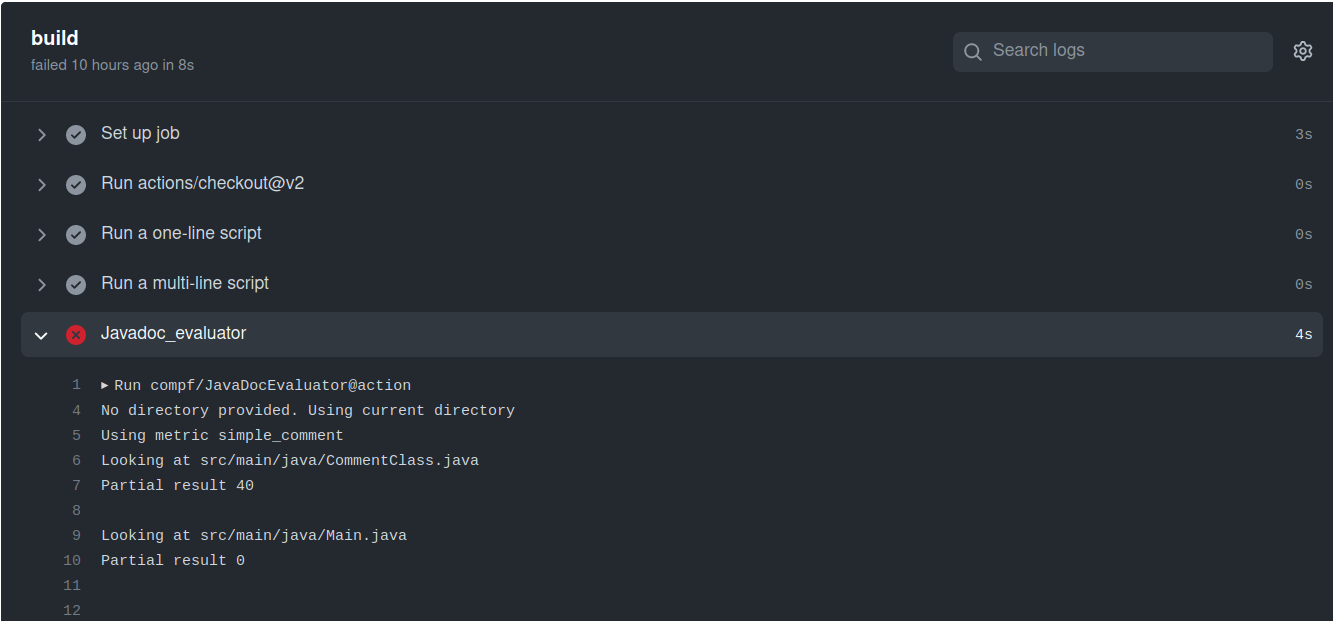
\includegraphics[width=\columnwidth]{figures/chapter2/workflow_output.png}
    \caption{Ausgabe eines Workflows}
    \label{fig:workflow_output}
\end{figure}

\subsubsection{Erstellung einer eigenen Action}
Um eine eigene GitHub Action zu erstellen, muss in dem Hauptverzeichnis des Repositorys, in dem der Programmcode der Action liegt, eine Datei namens \enquote{action.yaml} oder \enquote{action.yml} erstellt werden. Listing \ref{lst:create_action_example} zeigt eine beispielhafte \enquote{action.yaml}.
	\begin{figure}[h!]
			\lstinputlisting
			[caption={Beispielhafte Action-Konfigurationsdatei},
			label={lst:create_action_example},
			captionpos=b, basicstyle=\footnotesize, tabsize=1, showstringspaces=false,  numbers=left,language=YAML]
			{figures/chapter2/create_action_example.yaml}
		\end{figure}
Zunächst wird der Name der Action und eine Beschreibung definiert. Anschließend können Eingabeparameter definiert werden, die später im Programm verwendet werden können. Zu jedem Parameter muss auch festgelegt werden, ob er zwingend erforderlich ist und den Standardwert des Parameters. Außerdem können Ausgabeparameter festgelegt werden, die spätere Actions als Eingabe nutzen können. Danach wird festgelegt, wie diese Action ausgeführt wird. Eine Action kann in einer JavaScript-Umgebung, in einem Docker-Container, oder als Liste von verschiedenen Steps ausgeführt werden \cite[S. 117ff.]{github_action_book}. 


\section{Verwandte Werkzeuge}
Um die Qualität der Softwaredokumentation in Javadoc zu bewerten, gibt es bereits einige Programme. In vielen Fällen handelt es sich dabei um Programme, die nicht auf die Bewertung der Softwaredokumentation beschränkt sind, sondern auch andere Fälle von unsauberem Code erkennen können. Da die Bewertung der Dokumentation nicht der primäre Zweck der Programme ist, sind die verwendeten Metriken recht allgemein und erkennen viele Problemfälle nicht. Nichtsdestotrotz sind diese Programme, dadurch dass sie viele \enquote{Code-Smells} erkennen, gut geeignet, um sich ein gutes Bild über die Qualität des Quellcodes zu verschaffen und den Entwickler zu Clean-Code zu motivieren. 
\subsubsection{Checkstyle}
Eines der bekanntesten Programme ist Checkstyle \cite{Checkstyle}. Mit Checkstyle lässt sich beispielsweise prüfen, ob alle Methoden überhaupt ein Javadoc-Block besitzen, der Javadoc-Block korrekt platziert wurde oder ein Javadoc-Tag wie zum Beispiel \enquote{@deprecated} auch mit einer zusätzlichen Begründung versehen wurde. 
\subsubsection{PMD}
Des Weiteren gibt es das Programm PMD \cite{PMD}, das ebenfalls einige Metriken für Javadoc mitliefert. Dazu gehört, ob jede öffentliche Methode dokumentiert wurde oder die Kommentare generell zu lang sind. Interessanterweise gibt es auch die Möglichkeit, bestimmte Wörter, die als anstößig empfunden werden, aus Kommentaren und Dokumentationen auszuschließen, damit Kommentare neutral bleiben. 
\subsubsection{Javadoc}
Das oben erwähnte Javadoc-Tool bietet ebenfalls die Möglichkeit, beim Generieren der HTML-Datei die Qualität des Javadocs zu prüfen. Dabei werden vor allem fehlende Tags für Parameter etc. bemängelt. Zudem erkennt Javadoc auch Tabellen mit fehlender Überschrift und andere Designmängel, die in der HTML-Seite später auffallen. Auch fehlerhaftes HTML kann erkannt werden.

\section{Verwandte Arbeiten}

Neben den praktischen Tools, die den Softwareentwickler bei der Bewertung der Softwaredokumentation unterstützen, wurden auch einige wissenschaftliche Arbeiten veröffentlicht, die sich mit Metriken über Softwaredokumentation auseinandersetzen. In diesen Arbeiten werden auch Programme vorgestellt. welche diese Metriken nutzen, allerdings sind die Quelltexte bzw.  lauffähige Versionen der Programme ohne Weiteres nicht verfügbar, sodass ein Vergleich mit dem zu entwickelnden Tool nicht möglich ist. 


\subsubsection{Quasoledo}\label{chapter:Quasoledo}
In \cite[S. 4-10]{HowDocumentationEvolvesoverTime} geben die Autoren einige Metriken an, die sie für die Bewertung der Softwaredokumentation als nützlich erachten, und stellen ein Programm namens \enquote{}{Quasoledo} vor, dass mittels dieser Metriken Softwaredokumentationen analysieren kann. Zu den Metriken gehören z.~B.  \textit{ANYJ},  welches den Anteil der dokumentierten Deklarationen an allen Deklarationen beschreibt und \textit{KINCAID}, welches die Lesbarkeit von Texten beschreibt.

Die Arbeit wertet anschließend die Javadoc-Dokumentation von Eclipse aus und findet heraus, dass öffentliche Methoden häufiger dokumentiert sind und ihre Dokumentation oft lesbarer ist. Außerdem wenden die Autoren das Tool auf die gesamte Versionshistorie von Eclipse bis zum 8. April 2006 an und plotten den Verlauf der Dokumentationsqualität über diesem Zeitraum. Dabei wird sichtbar, dass die Qualität am Anfang des Projektes noch sehr stark schwankt, aber nach einiger Zeit recht konstant bleibt. 
\subsubsection{JavaDocMiner}
Eine weitere Arbeit, die eine der Grundlagen dieser Bachelorarbeit ist, ist der \enquote{JavaDocMiner} \cite[S. 68-79]{AutomaticQualityAssessmentofSourceCodeComments:TheJavadocMiner}. In diesem Konferenzpapier wird ein Programm beschrieben, welches mittels einfacher Heuristiken eine Einschätzung der Softwaredokumentation beschrieben. Das Tool extrahiert aus XML-Dateien, die mittels eines selbst geschriebene Doclet aus Javadoc erstellt wurden, die notwendigen Informationen und wendet dann auf diese XML-Struktur die Metriken an. 

Insgesamt verwendeten die Autoren viele Metriken aus dem Tool \hyperref[chapter:Quasoledo]{Quasoledo}, führen aber neue auch Metriken ein, die Anzahl der Abkürzungen zählen, da diese laut der Arbeit vermieden werden sollten. Auch die durchschnittliche Anzahl an Wörtern pro Javadoc-Kommentar wird als Metrik verwendet. 

Anschließend wendeten die Autoren das Tool auf den Quellcode an und prüften, ob es eine Korrelation zwischen der Anzahl an Bugs und der Qualität der Dokumentation nach den benannten Metriken und fanden dabei heraus, dass die Kincaid-Metrik nur wenig mit der Anzahl der Bugs korreliert, während es bei anderen Metriken wie z.~B. \textit{ANYJ} eine starke negative Korrelation gab. 

\subsubsection{Doc2Spec}
Die Autoren in \cite[S. 307ff.]{InferringResourceSpecificationsfromNaturalLanguageAPIDocumentation} stellen ein Tool namens \enquote{Doc2Spec} vor und erläutern ein Verfahren, um herauszufinden, ob eine API korrekt verwendet wurde. Dabei werden die Javadoc-Kommentare einer API analysiert und dann mit der Verwendung der API verglichen, um Fehler bei der Handhabung der API zu finden. 

Für jede dokumentierte Methode der API wird ein Aktion-Ressource-Paar erstellt. Diese beschreibt, welche Aktion auf welche Ressource ausgeführt wird. Bei einer Methode namens \textit{close}, die mit dem englischen Text \enquote{Initiates close of the connection handle at the
application level} dokumentiert wird, lässt sich beispielsweise schlussfolgern, dass das Aktion-Ressource-Paar \textit{(close,connection)} sein kann; denn die Aktion \textit{close} bezieht sich auf die Ressource \textit{connection}. Dabei sind aber manchmal mehrere Aktion-Ressource-Paare möglich \cite[S. 308]{InferringResourceSpecificationsfromNaturalLanguageAPIDocumentation}.

Anschließend werden die gefundenen Ressourcen anhand der Klassenhierarchie passend gruppiert. Außerdem werden die Aktionen in fünf Kategorien eingeordnet, in der die meisten Java-Methoden passen. Die Kategorien sind Methoden, die eine Ressource oder Objekt erstellen, eine Ressource sperren, auf eine Ressource zugreifen, eine gesperrte Ressource wieder freigeben und Ressourcen schließen. 

Mit diesen generierten Informationen kann dann bei Quelltext, welches diese API verwendet, geprüft werden, ob die Methoden dieser Ressource in der richtigen Reihenfolge aufgerufen werden. Beispielsweise muss eine Ressource zuerst erzeugt und gesperrt werden, bevor irgendwelche Manipulationen angewendet werden. Außerdem kann geprüft werden, ob eine Ressource auch wieder freigegeben und geschlossen wird, sodass Speicherlecks verhindert werden. Dabei werden alle möglichen Ausführungspfade einer Methode geprüft, da ein fehlendes Freigeben von Ressourcen z.~B. im Ausnahmefall ein häufiger Fehler sein kann. 
\begin{comment}
\subsubsection{iComment}
Das Programm \enquote{iComment}  wurde hauptsächlich für C-Programme entwickelt, um Probleme zwischen der Dokumentation und dem Quellcode zu finden. Dabei konzentriert sich das Programm auf das Finden von Synchronisationsproblemen, die bei Programmen mit mehreren Threads auftauchen können.  Bei einem exklusiven Ausschluss besitzt eine Methode einen sogenannten Lock auf ein Objekt und nur diese Methode darf mit dem Objekt arbeiten.

Setzt nun die Dokumentation einen Lock voraus, aber der Programmierer hat keinen Lock angefordert, können sehr schnelle und subtile Bugs entstehen, die nur schwer findbar sind. \cite[S. 145ff.]{icomment}

Das Programm wurde auf dem Quellcode des Linux-Kernels und Mozilla angewandt und dabei mögliche Bugs gefunden, die später auch von den Entwicklern bestätigt wurden\cite[S. 146.]{icomment}.

\end{comment}
\subsubsection{@tComment}\label{@tComment}
Ein anderer Ansatz, der ebenfalls mit Javadoc arbeitet, wird \enquote{@tComment} genannt \cite[S. 1ff.]{@tComment:TestingJavadocCommentstoDetectComment-CodeInconsistencies}. Dabei wurde die Konsistenz der Javadoc-Dokumentation mit dem tatsächlichen Programmcode verglichen. Anders als die vorherigen Ansätze, wird hier das Programm dynamisch ausgeführt. Dabei werden die verschiedenen Methoden und ihr dazugehörige Javadoc-Dokumentation analysiert und daraus mittels einfacher Heuristiken ermittelt, ob ein  Nullwert für einen Parameter eine Inkonsistenz zwischen Dokumentation und Quellcode offenbart.

Beispielsweise kann die Dokumentation einer Java-Methode beschreiben, dass ein Parameter nicht null sein darf. Daraus kann gefolgert werden, dass ein Nullwert für diesen Parameter zu einer Ausnahme führt. Wenn diese Ausnahme dann auch genauer in der Dokumentation genauer spezifiziert ist, sollte genau diese Ausnahme bei einem Nullwert geworfen werden. 

Falls Nullwerte explizit erlaubt sind, sollte die Methode sich dann stets korrekt verhalten und keine Ausnahmen werfen. 

\enquote{@tComment} kann mit diesen einfachen Regeln jede Methode ausführen und prüfen, ob sich die Methode tatsächlich verhält, wie die Dokumentation es beschreibt. Dabei verwendet das Programm einfache \ac{NLP}-Heuristiken in der englischen Sprache; zum Beispiel prüft das Programm, ob die kurz vor dem Wort \enquote{null} ein negierendes Wort wie \enquote{not} oder \enquote{never} auftaucht und klassifiziert dann den dazugehörigen Parameter als Parameter, der nie null sein darf. 
